% #############################################################################
% This is Chapter 5
% !TEX root = ../main.tex
% #############################################################################
% Change the Name of the Chapter i the following line
\fancychapter{Implementation}
\cleardoublepage
% The following line allows to ref this chapter
\label{chap:solution}

Symmetric keys will be used to encrypt and authenticate messages. They have better performance with larger messages compared to asymmetric keys. Each user can have stored in their box, several symmetric keys. This enables the user to establish secure communications with multiple different people or groups.
The non-repudiation property of asymmetric keys will be used to create digital signatures of documents. The other use, will be to share symmetric keys between user who wish to communicate. The box stores the private and public key pair of the user, and the public keys of people the user wishes to trade secrets with.

% -----------------------------------------------------
% -----------------------------------------------------
\section{Initial State}\label{chap:solution:initial-state}

The entities will receive the device with a pair of asymmetric keys, a private and public, generated inside the device from fabric. Each device will have the user's public keys, whom he wishes to communicate. The entity can request whose public keys he wants, before the device is initialized in fabric. This allows the users to share symmetric keys between them, which they can user to begin trading data securely. The device can also come with the symmetric keys already shared and stored in each user device.
For each user or group a user wants to communicate with, he has a symmetric key stored in the device.

% -----------------------------------------------------
% -----------------------------------------------------
\section{Protocol}\label{chap:solution:protocol}

This section will explain and define the communication protocols between both components in more detail. For each operation, it will describe the different phases, what data is traded and why.

\subsection{Device Standardization}

The solution should work with a plethora of devices, which will increase the adoptability of the solution among clients. This entails the use of a widely established protocol, which clearly defines a set of functions and standards the system should follow.
This is where the \ac{PKCS} \#11 standard is again relevant. It allows operations to be standardized across different devices, increasing the range of supported devices. By implementing the system in accordance with these guidelines, it will have a higher device interoperability.

% -----------------------------------------------------
\subsection{Authentication Protocol}\label{chap:solution:protocol:auth}

%% Insert protocol image here
\begin{figure}[h]
	\centering
	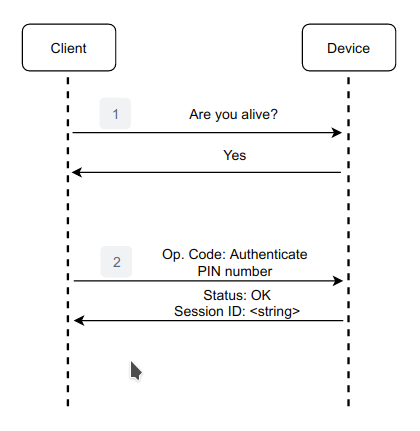
\includegraphics[width=0.5\textwidth]{./Images/authentication.png}
	\caption{Authentication Protocol}
	\label{fig:protocol:authentication}
\end{figure}

Before executing any operation the user must authenticate himself to the device.
The protocol described is pictured in figure~\ref{fig:protocol:authentication}.

\begin{enumerate}
	\item The first phase is initiated by the user by sending a message to check if the box is alive and connected to the computer.
	\item The operation will move to the second phase when the user receives an affirmative response. He will then send the operation code, which indicates he wants to authenticate himself, and the authentication \ac{PIN}. The device will respond with a status parameter indicating failure or success. When successful the session between the user and the box will be unlocked, allowing the user to do other operations.
\end{enumerate}

%% TODO - in case I decide to keep the session ID, add paragraph explaining how it is used in all operations, else delete this

% -----------------------------------------------------
\subsection{Administration Protocol}\label{chap:solution:protocol:admin}
%% Insert protocol image here
\begin{figure}[h]
	\centering
	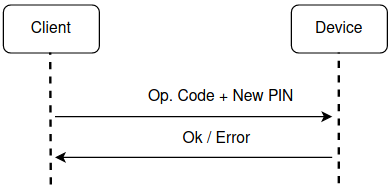
\includegraphics[width=0.5\textwidth]{./Images/change-PIN.png}
	\caption{Change Authentication PIN protocol}
	\label{fig:protocol:change-PIN}
\end{figure}

As explained before, there is only one administration operation, changing the authentication \ac{PIN}, pictured in figure~\ref{fig:protocol:change-PIN}.

The user initiates by sending the operation code, identifying the operation and the new \ac{PIN} number. The device responds with the success or failure of the operation.

% -----------------------------------------------------
\subsection{Data Exchange Protocol}\label{chap:solution:protocol:data}

%% Insert protocol image here
\begin{figure}[h]
	\centering
	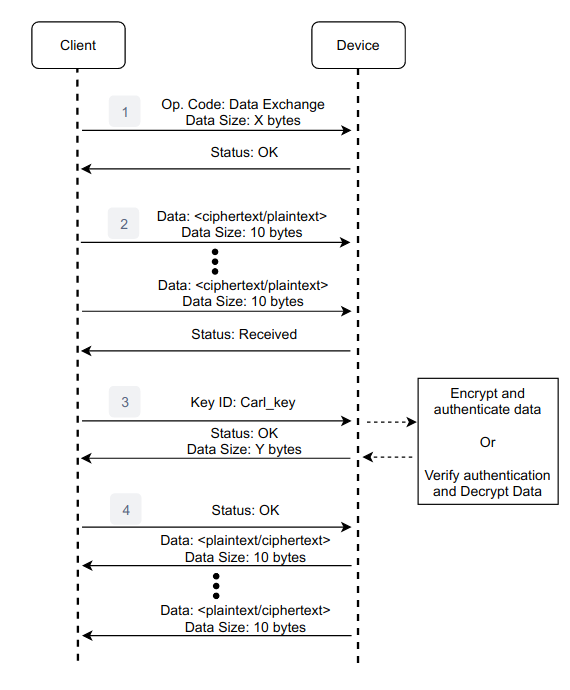
\includegraphics[width=0.6\textwidth]{./Images/data-exchange.png}
	\caption{Data Exchange Encryption Protocol}
	\label{fig:protocol:data-exchange}
\end{figure}

The protocol to encrypt and authenticate data illustrated in figure~\ref{fig:protocol:data-exchange} consists of:
\begin{enumerate}
	\item The user sends the operation code and the data size, signaling he wants to send some data;
	\item The box will respond with an OK message that the user can begin transmitting the data. It will be transmitted a maximum of X bytes per `packet'. Each packet contains a part of the data and the size of the data in that packet. When the transmission ends, the device will confirm its reception;
	\item The user subsequently will respond with the symmetric key ID, which he wants to encrypt and authenticate the data with. The box will handle the cryptographic operations and return a status message and the encrypted data size.
	\item After the client confirms, the encrypted data with the additional MAC and IV parameters appended, will be returned in the same manner it was sent.
\end{enumerate}

The protocol to decrypt and verify data authentication is very similar to the previous one, and is also pictured in figure~\ref{fig:protocol:data-exchange}.

\begin{enumerate}
	\item The operation code is sent, as well as the encrypted data size;
	\item The box will respond with an OK message that the user can begin transmitting the data, one packet at a time;
	\item When the data transmission ends, the device will confirm its reception, and the user will subsequently respond with the symmetric key ID, which can decrypt and verify the data authentication;
	\item After performing the decryption and authentication operations, the device will return a message indicating its success or failure. In case of a successful operations, it will return, in the same manner it was sent, the plaintext data.
\end{enumerate}

In the case of digital signatures, the user's must have each others public keys, if they do not already have them.

%% --------------------------
%% Insert protocol image here
\begin{figure}[h]
	\centering
	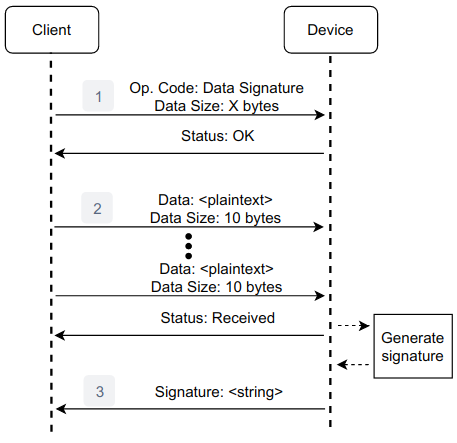
\includegraphics[width=0.6\textwidth]{./Images/signature-generate.png}
	\caption{Digital Signature Generation}
	\label{fig:protocol:signature-generate}
\end{figure}

The next protocols are relating to the generation and verification of digital signatures.
The designed protocol for generation is represented in figure~\ref{fig:protocol:signature-verify}.

% \begin{enumerate}
%         \item The user initiates with the code operation and the plaintext data size;
%         \item When the box responds with an OK message, the user transmits the data one packet at a time;
%         \item In possession of the data, the device will generate the digital signature using the user's private key. When finished the signature is sent back.
% \end{enumerate}
The user initiates by sending the operation code and the plaintext data size.
When the box responds with an OK message, the user transmits the data to be signed, one packet at a time.
In possession of the data, the device will generate the digital signature using the user's private key. When finished the signature is sent back to the user.

%% ----------------------------------------
%% Insert protocol image here
\begin{figure}[h]
	\centering
	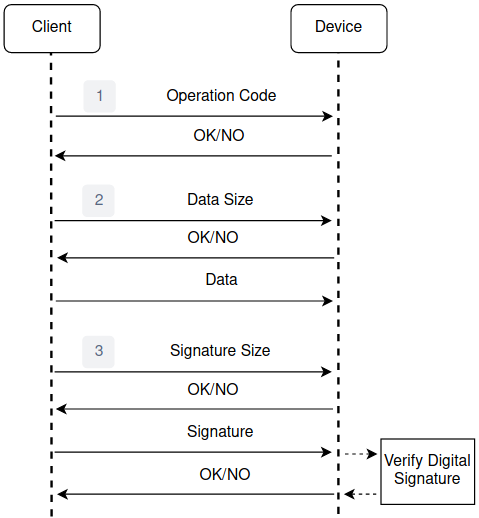
\includegraphics[width=0.6\textwidth]{./Images/signature-verify.png}
	\caption{Digital Signature Verification}
	\label{fig:protocol:signature-verify}
\end{figure}

The protocol for verifying digital signatures is pictured in figure~\ref{fig:protocol:signature-verify}.

% \begin{enumerate}
%         \item The user initiates with the code operation;
%         \item When the box responds with an OK message, the user transmits the data one packet at a time;
%         \item When done, the user also sends the signature and the name of the signer, so the device knows what public key to use to verify the signature;
%         \item Then, the device will verify the digital signature using the signer's public key, data and signature. The result will be sent back to the user.
% \end{enumerate}
After the user sends the operation code, and the box responds with an OK message, the user transmits the data, used by the signer to generate the signature, one packet at a time.
When done, the user also sends the signature and the name of the signer, so the device knows what public key to use to verify the signature.
Then, the device will verify the digital signature using the signer's public key, the data and the signature. The result will be sent back to the user.

% -----------------------------------------------------
\subsection{Key Exchange Protocol}\label{chap:solution:protocol:key}

%% Insert protocol image here
\begin{figure}[h]
	\centering
	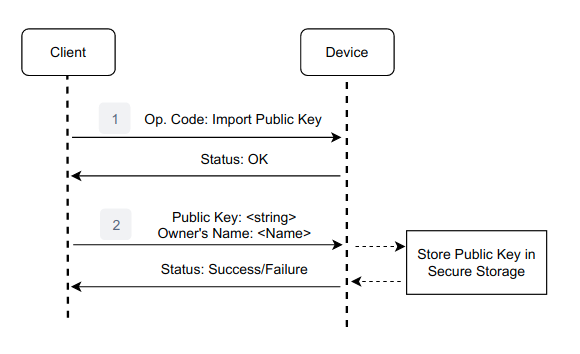
\includegraphics[width=0.6\textwidth]{./Images/import-pub-key.png}
	\caption{Import Public Key}\label{fig:protocol:import-pub}
\end{figure}

Starting with the import public keys protocol, also represented in figure~\ref{fig:protocol:import-pub}.
% \begin{enumerate}
%         \item The user send a message with the operation code, indicating he wants to send someone's public key;
%         \item After the device responds with an OK signal, the user sends the public key, and the name of the owner of the public key;
%         \item The device then informs the user of the operation's success or failure.
% \end{enumerate}
The user send a message with the operation code, indicating he wants to store someone's public key.
After the device responds with an OK signal, the user sends the public key, and the name of the owner of the public key.
The device, stores the public key, associated to the name sent by the user, and informs the user of the operation's success or failure.

%% -------------------------------------
Just like digital signatures, for users to be able to share symmetric keys between each other, they must possess each others public keys in their device. If not, they must physically meet to share them, and import them to their respective devices, with the available operation.

%% Insert protocol image here
\begin{figure}[h]
	\centering
	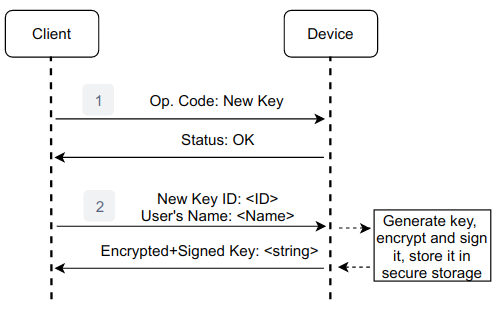
\includegraphics[width=0.6\textwidth]{./Images/new-key.png}
	\caption{Protocol to generate new key to share with user.}
	\label{fig:protocol:new-key}
\end{figure}

The protocol to generate a new symmetric key, and securely share it with a user is represented in figure~\ref{fig:protocol:new-key}.
% \begin{enumerate}
%         \item The user sends a message with the operation code;
%         \item After the device responds with an OK signal, the user sends the key ID, the name the key will be saved as, and the name of the user he wants to share the key with, so the device knows which public key to use to secure the key;
%         \item A new symmetric key will be generated and saved in the device's secure storage, with the key ID sent by the user. The box will encrypt and sign the key with public-key cryptography, and send it to the user, which he can securely share with the other user.
% \end{enumerate}
The user sends a message with the operation code.
After the device responds with an OK signal, the user sends the key ID, the name the key will be saved as, and the name of the user he wants to share the key with, so the device knows which public key to use to secure the key.
A new symmetric key will be generated and saved in the device's secure storage, with the key ID sent by the user. The box will encrypt and sign the key with public-key cryptography, and send it to the user, which he can securely share with the other user.

%% Insert protocol image here
\begin{figure}[h]
	\centering
	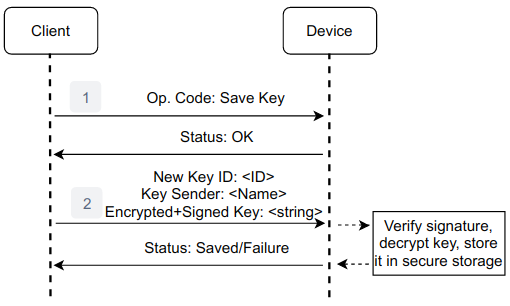
\includegraphics[width=0.6\textwidth]{./Images/save-key.png}
	\caption{Protocol to save key, received from another user.}
	\label{fig:protocol:save-key}
\end{figure}

The protocol for the other user to save the newly received symmetric key, and store it inside their device is in figure~\ref{fig:protocol:save-key}.

% \begin{enumerate}
%         \item The user sends a message with the operation code;
%         \item After the device responds with an OK signal, the user sends the key ID, the name of the key sender, and the encrypted and signed key;
%         \item The device will then verify the signature with the sender's public key and decrypt the key, subsequently saving it in the device's secure storage along with other keys already present.
% \end{enumerate}
After the operations code is sent and the OK signal is returned, the user sends the key ID, the name of the key sender, and the encrypted and signed key.
The device will then verify the signature with the sender's public key and decrypt the key, subsequently saving it in the device's secure storage along with other keys already present.
